\documentclass{article}
%%%%%%%%%%%%%%%%%%%%%%%%%%%%%%%%%%%%%%%%%%%%%%%%%%%%%%%%%%%%%%%%%%
%%%%%%%%%%%%%%%%%%%%%%%%%%%%%%%%%%%%%%%%%%%%%%%%%%%%%%%%%%%%%%%%%%
%Packages
\usepackage[top=3cm, bottom=3cm, left=2.5cm, right=2.5cm]{geometry}
\usepackage{amsmath,amsthm,amsfonts,amssymb,amscd, fancyhdr, color, comment, graphicx, environ}
\usepackage{float}
\usepackage{mathrsfs}
\usepackage[math-style=ISO]{unicode-math}
\setmathfont{TeX Gyre Termes Math}
\usepackage{lastpage}
% \usepackage[dvipsnames]{xcolor}
\usepackage[table]{xcolor}
\usepackage[framemethod=TikZ]{mdframed}
\usepackage{enumerate}
\usepackage[shortlabels]{enumitem}
\usepackage{fancyhdr}
\usepackage{indentfirst}
\usepackage{listings}
% \usepackage{sectsty}
\usepackage{thmtools}
\usepackage{shadethm}
\usepackage{hyperref}
\usepackage{setspace}
\usepackage{datetime}
\usepackage{shadethm}
\usepackage{lipsum}
\usepackage{blindtext}
\usepackage[base]{babel}
\usepackage{xparse}
\usepackage{changepage}
\usepackage{tabularx}
\usepackage{multirow}
\usepackage{colortbl}
\usepackage[fontsize=12pt]{fontsize}
\hypersetup{
    colorlinks=true,
    linkcolor=brown,
    filecolor=magenta,      
    urlcolor=brown,
}

%%%%%%%%%%%%%%%%%%%%%%%%%%%%%%%%%%%%%%%%%%%%%%%%%%%%%%%%%%%%%%%%% Assignment Number
\newcommand\hwnumber{1}    % <-- homework number

%%%%%%%%%%%%%%%%%%%%%%%%%%%%%%%%%%%%%%%%%%%%%%%%%%%%%%%%%%%%%%%%%% Colors
\definecolor{mGreen}{rgb}{0,0.6,0}
\definecolor{mGray}{rgb}{0.5,0.5,0.5}
\definecolor{mPurple}{rgb}{0.58,0,0.82}
\definecolor{backgroundColour}{rgb}{0.98,0.98,0.95}

%%%%%%%%%%%%%%%%%%%%%%%%%%%%%%%%%%%%%%%%%%%%%%%%%%%%%%%%%%%%%%%%%%
%%%%%%%%%%%%%%%%%%%%%%%%%%%%%%%%%%%%%%%%%%%%%%%%%%%%%%%%%%%%%%%%%%
%Environment setup
\mdfsetup{skipabove=\topskip,skipbelow=\topskip}
\newrobustcmd\ExampleText{%
An \textit{inhomogeneous linear} differential equation has the form
\begin{align}
L[v] = f,
\end{align}
where $L$ is a linear differential operator, $v$ is the dependent
variable, and $f$ is a given non−zero function of the independent
variables alone.
}

\mdtheorem[style=theoremstyle]{Problem}{Part}
\newenvironment{Solution} {
\begin{large}
    \textbf{Solution.}
\end{large}
\vspace{4pt}
\par
}

%%%%%%%%%%%%%%%%%%%%%%%%%%%%%%%%%%%%%%%%%%%%%%%%%%%%%%%%%%%%%%%%%%
%%%%%%%%%%%%%%%%%%%%%%%%%%%%%%%%%%%%%%%%%%%%%%%%%%%%%%%%%%%%%%%%%%
%Fill in the appropriate information below
\newcommand{\norm}[1]{\left\lVert#1\right\rVert} 
\newcommand\course{ESO207A}                      % <-- course name   
\newcommand\RollNumber{200259}  % <-- personal information
\newcommand\image{images/CS422.png}
\newcommand\numberthis{\addtocounter{equation}{1}\tag{\theequation}} % number needed equation in align
%%%%%%%%%%%%%%%%%%%%%%%%%%%%%%%%%%%%%%%%%%%%%%%%%%%%%%%%%%%%%%%%%%
%%%%%%%%%%%%%%%%%%%%%%%%%%%%%%%%%%%%%%%%%%%%%%%%%%%%%%%%%%%%%%%%%%
%Page setup
\lstset{language=C, keywordstyle={\bfseries \color{blue}}}
\pagestyle{fancy}
\headheight 35pt
\lhead{\begin{Large}Assignment \hwnumber\end{Large}}
\rhead{\includegraphics[width=2cm]{\image}}
\lfoot{}
\pagenumbering{arabic}
\cfoot{\small\thepage}
\rfoot{}

\mdfdefinestyle{theoremstyle}{%
linecolor=black,linewidth=1pt,%
frametitlerule=true,%
frametitlebackgroundcolor=gray!20,
innertopmargin=\topskip,
innerbottommargin=\topskip
}
%%%%%%%%%%%%%%%%%%%%%%%%%%%%%%%%%%%%%%%%%%%%%%%%%%%%%%%%%%%%%%%%%%
%%%%%%%%%%%%%%%%%%%%%%%%%%%%%%%%%%%%%%%%%%%%%%%%%%%%%%%%%%%%%%%%%%
%Add new commands here
\renewcommand{\labelenumi}{\alph{enumi})}
\newcommand{\Z}{\mathbb Z}
\newcommand{\R}{\mathbb R}
\newcommand{\Q}{\mathbb Q}
\newcommand{\NN}{\mathbb N}
\DeclareMathOperator{\Mod}{Mod} 
\renewcommand\lstlistingname{Algorithm}
\renewcommand\lstlistlistingname{Algorithms}
\def\lstlistingautorefname{Alg.}
\lstdefinestyle{CStyle}{
    backgroundcolor=\color{backgroundColour},   
    commentstyle=\color{mGreen},
    keywordstyle=\color{magenta},
    numberstyle=\tiny\color{mGray},
    stringstyle=\color{mPurple},
    basicstyle=\footnotesize,
    breakatwhitespace=false,         
    breaklines=true,                 
    captionpos=b,                    
    keepspaces=true,                 
    numbers=left,                    
    numbersep=5pt,                  
    showspaces=false,                
    showstringspaces=false,
    showtabs=false,                  
    tabsize=2,
    language=C
}
\NewDocumentCommand{\codeword}{v}{%
\texttt{\textcolor{blue}{#1}}%
}
\newdate{date}{25}{09}{2023}
%%%%%%%%%%%%%%%%%%%%%%%%%%%%%%%%%%%%%%%%%%%%%%%%%%%%%%%%%%%%%%%%%
% Begin now!
\begin{document}
%%%%%%%%%%%%%%%%%%%%%%%%%%%%%%%%%%%%%%%%%%%%%%%%%%%%%%%%%%%%%%%%%
% Title Page
\begin{titlepage}
    \begin{center}
        \vspace*{3cm}
            
        \Huge
        \textbf{Assignment \hwnumber}
            
        \vspace{3pt}
        
        \huge
        Analyze \texttt{ia-32} compiled SPEC-2006 \\ Benchmark Suite
        
        \vspace{40pt}
            
        \Large
        \textbf{Anshuman Barnwal} $\cdot$ \textbf{\RollNumber}
        
            
        \vfill
        
        Homework Assignment of
            
        \vspace{7pt}
            
        \includegraphics[width=0.4\textwidth]{\image}
        \\
        
        \Large
        
        \displaydate{date}
        
        \vspace{7pt}
            
    \end{center}
\end{titlepage}

%%%%%%%%%%%%%%%%%%%%%%%%%%%%%%%%%%%%%%%%%%%%%%%%%%%%%%%%%%%%%%%%%
% Start the assignment now
% Some extra information!
\newpage

\addcontentsline{toc}{section}{Background}
\section*{BACKGROUND}
You will analyze a subset of the SPEC 2006 benchmark suite compiled for the \texttt{ia32} (32-bit Intel architecture) ISA. Specifically, you will instrument each SPEC 2006 application binary with PIN and extract the percentages of various different instruction types. You will also use a very simple cycle accounting model to calculate the CPI for each application. Additionally, you will calculate the instruction and data footprints of each application. Finally, you will understand a few properties of the \texttt{ia32} ISA.

In this assignment, we will be interested only in the following instruction types. At a very high level, we have two instruction types.

\vspace{10pt}
\noindent
Type A: Instructions with no memory operand \\
Type B: Instructions with at least one memory operand
\vspace{10pt}

You should only instrument the instructions that actually execute i.e., have true predicates. As a result, you should always use $\texttt{INS\_InsertPredicatedCall}$ method when classifying instructions.

For Type B Instructions, Each memory operand in such an instruction can be read and/or written to.

We will view each such load or store operation within a type B instruction as a separate micro-instruction and count it as a separate instruction.

For example, a type B instruction may have two load operations and a store operation. Further, each such load or store operation may access an arbitrary amount of data. However, in a 32-bit processor, it is not possible to transfer more than 32 bits of data in one shot. As a result, we will further break down each memory operation into several memory accesses of size at most 32 bits.

Finally, the instruction must be using these memory operands to carry out some operation of type A. This operation should be counted as a separate type A instruction and should also be categorized into one of the fifteen categories mentioned above.

Let us take an example of an x86 instruction that has three memory operands, two of which are loads and one is a store. The loads access one and ten bytes, respectively. The store accesses eleven bytes. This instruction will be accounted as follows.

\vspace{10pt}
\noindent
\texttt{Number of loads:   4}\\
\texttt{Number of stores:   3}\\
\texttt{Number of type A instruction:  1}
\vspace{10pt}

\noindent
Total instruction count increases by eight, whenever such an instruction is encountered.

%%%%%%%%%%%%%%%%%%%%%%%%%%%%%%%%%%%%%%%%%%%%%%%%%%%%%%%%%%%%%%%%%
% Tasks pages begin
\newpage
\addcontentsline{toc}{section}{Tasks}
\section*{TASKS}

%%%%%%%%%%%%%%%%%%%%%%%%%%%%%%%%%%%%%%%%%%%%%%%%%%%%%%%%%%%%%%%%%
% New problem
\begin{Problem}
For each benchmark application, you need to report the dynamic counts and percentages of the following seventeen types of instructions. The total number of instructions (to be used as the denominator in the percentage) is the addition of all these seventeen counters. \\

% \includegraphics[width=0.9\textwidth]{./images/CS422_QuestionA.png}

Prepare a table showing these counts and percentages for the applications.
\end{Problem}

\begin{Solution}

\begin{figure}[H]
    \centering
    \includegraphics[width=0.9\textwidth]{images/CS422_QuestionA.png}
    \caption{Types of Instructions (Load-Store may overlap others)}
    \label{fig:pA:partitions}
\end{figure}

All the benchmark applications provided were fast-forwarded by a given number of instructions. During fast-forwarding, consider each instruction irrespective of type, as $1$ instruction while in instrumentation period, considered every instruction containing $n$ 32b loads and $m$ 32b stores components as equivalent to $1 + n + m$ instructions.

\vspace{10pt}
The below tables store the required data regarding all type of instructions. ``Percent" is the corresponding $\frac{\text{Count}}{\text{Effective}}$ where ``Effective" is as in \ref{tab:pA:instruction_counts}.

We found ``Vector Instructions", ``Conditional Moves", ``MMX and SSE Instructions", and ``System Calls" to be $0$ for all the applications.

Below at \ref{tab:pA:floating_rest_counts}, Memory Instructions is essentially Loads and Stores together.

\begin{table}[!htbp]
\centering
\caption{Actual \#Instruction v/s Effective $1 + n + m$ \#Instruction and their ratio}
\label{tab:pA:instruction_counts}
\begin{tabular}{| l | c | >{\columncolor[gray]{0.8}}c | >{\columncolor[gray]{0.8}}c | c |}
\hline
\multirow{2}{*}{Application} & \multirow{2}{*}{FastForward$^{(B)}$} & \multicolumn{2}{c|}{Instruction Counts} & \multirow{2}{*}{Percentage} \\
\cline{3-4}
& & Actual & Effective & \\
\hline
400.perlbench & 207 & 643629926 & 999864910 & 64.37\% \\
\hline
401.bzip2 & 301 & 626757711 & 999997068 & 62.67\% \\
\hline
403.gcc & 107 & 694478005 & 999992310 & 69.45\% \\
\hline
429.mcf & 377 & 660698717 & 1000000000 & 66.07\% \\
\hline
450.soplex & 364 & 615283889 & 1000000001 & 61.53\% \\
\hline
456.hmmer & 264 & 616007786 & 999999444 & 61.60\% \\
\hline
471.omnetpp & 43 & 625784586 & 1000000000 & 62.58\% \\
\hline
483.xalancbmk & 1331 & 652390226 & 999688603 & 65.26\% \\
\hline
\end{tabular}
\end{table}

\begin{table}[!htbp]
\centering
\caption{Load and Store \#Instructions}
\label{tab:pA:load_store_counts}
\begin{tabular}{| l | >{\columncolor[gray]{0.8}}c | c | >{\columncolor[gray]{0.8}}c | c |}
\hline
\multirow{2}{*}{Application} & \multicolumn{2}{c|}{Loads} & \multicolumn{2}{c|}{Stores} \\
\cline{2-3}\cline{4-5}
& Count & Percent & Count & Percent \\
\hline
400.perlbench & 235396718 & 23.543 & 120973356 & 12.099 \\
\hline
401.bzip2 & 286663856 & 28.666 & 86578433 & 8.658 \\
\hline
403.gcc & 22555350 & 2.255 & 282966645 & 28.301 \\
\hline
429.mcf & 274762679 & 27.476 & 64538604 & 6.459 \\
\hline
450.soplex & 335145819 & 33.514 & 49570293 & 4.957 \\
\hline
456.hmmer & 337431712 & 33.743 & 46560502 & 4.656 \\
\hline
471.omnetpp & 232166088 & 23.217 & 142049326 & 14.205 \\
\hline
483.xalancbmk & 239302390 & 23.938 & 108307384 & 10.834 \\
\hline
\end{tabular}
\end{table}

\begin{table}[!htbp]
\centering
\caption{NOP, Direct and Indirect Calls \#Instructions}
\label{tab:pA:nop_calls_counts}
\begin{tabular}{| l | >{\columncolor[gray]{0.8}}c | c | >{\columncolor[gray]{0.8}}c | c | >{\columncolor[gray]{0.8}}c | c |}
\hline
\multirow{2}{*}{Application} & \multicolumn{2}{c|}{NOPs} & \multicolumn{2}{c|}{Direct Calls} & \multicolumn{2}{c|}{Indirect Calls} \\
\cline{2-3}\cline{4-5}\cline{6-7}
& Count & Percent & Count & Percent & Count & Percent \\
\hline
400.perlbench & 433528 & 0.0433 & 6947662 & 0.695 & 2165028 & 0.216 \\
\hline
401.bzip2 & 32147 & 0.00321 & 11032 & 0.00110 & 0 & 0.000 \\
\hline
403.gcc & 90112 & 0.00901 & 1275299 & 0.128 & 13555 & 0.00136 \\
\hline
429.mcf & 879752 & 0.0879 & 8266384 & 0.826 & 0 & 0.000 \\
\hline
450.soplex & 1852 & 0.00018 & 2374689 & 0.237 & 54 & 0.0000 \\
\hline
456.hmmer & 14312 & 0.0014 & 86688 & 0.0087 & 553 & 0.00005 \\
\hline
471.omnetpp & 503202 & 0.0503 & 13391515 & 1.339 & 2307982 & 0.231 \\
\hline
483.xalancbmk & 14237079 & 1.424 & 8707590 & 0.871 & 5826909 & 0.583 \\
\hline
\end{tabular}
\end{table}

\begin{table}[!htbp]
\centering
\caption{Returns, Unconditional and Conditional Branches \#Instructions}
\label{tab:pA:ret_branch_counts}
\begin{tabular}{| l | >{\columncolor[gray]{0.8}}c | c | >{\columncolor[gray]{0.8}}c | c | >{\columncolor[gray]{0.8}}c | c |}
\hline
\multirow{2}{*}{Application} & \multicolumn{2}{c|}{Returns} & \multicolumn{2}{c|}{Uncond. Branches} & \multicolumn{2}{c|}{Cond. Branches} \\
\cline{2-3}\cline{4-5}\cline{6-7}
& Count & Percent & Count & Percent & Count & Percent \\
\hline
400.perlbench & 9112689 & 0.911 & 20172634 & 2.017 & 82678603 & 8.268 \\
\hline
401.bzip2 & 11031 & 0.0011 & 14741341 & 1.474 & 84526720 & 8.453 \\
\hline
403.gcc & 1288855 & 0.128 & 1488031 & 0.148 & 97945541 & 9.794 \\
\hline
429.mcf & 8266383 & 0.826 & 5572158 & 0.557 & 117749486 & 11.77 \\
\hline
450.soplex & 2374743 & 0.237 & 7571500 & 0.757 & 64241385 & 6.424 \\
\hline
456.hmmer & 87241 & 0.0087 & 113915 & 0.0113 & 88919715 & 8.891 \\
\hline
471.omnetpp & 15699500 & 1.569 & 13881657 & 1.388 & 73391837 & 7.339 \\
\hline
483.xalancbmk & 14538758 & 1.454 & 5687717 & 0.568 & 115456999 & 11.549 \\
\hline
\end{tabular}
\end{table}

\begin{table}[H]
\centering
\caption{Logical, Rotate-Shift and Flag Operations \#Instructions}
\label{tab:pA:logic_flag_counts}
\begin{tabular}{| l | >{\columncolor[gray]{0.8}}c | c | >{\columncolor[gray]{0.8}}c | c | >{\columncolor[gray]{0.8}}c | c |}
\hline
\multirow{2}{*}{Application} & \multicolumn{2}{c|}{Logical Op} & \multicolumn{2}{c|}{Rotate \& Shift} & \multicolumn{2}{c|}{Flag Op} \\
\cline{2-3}\cline{4-5}\cline{6-7}
& Count & Percent & Count & Percent & Count & Percent \\
\hline
400.perlbench & 61151842 & 6.116 & 2897866 & 0.289 & 478094 & 0.0478 \\
\hline
401.bzip2 & 51058392 & 5.105 & 44677195 & 4.467 & 4398 & 0.0004 \\
\hline
403.gcc & 94626225 & 9.462 & 917464 & 0.0917 & 36715 & 0.0036 \\
\hline
429.mcf & 49278688 & 4.927 & 2313100 & 0.231 & 0 & 0.000 \\
\hline
450.soplex & 8780117 & 0.878 & 6691975 & 0.669 & 13408915 & 1.340 \\
\hline
456.hmmer & 692045 & 0.0692 & 167329 & 0.0167 & 2879 & 0.0002 \\
\hline
471.omnetpp & 37629094 & 3.762 & 4483798 & 0.448 & 12598264 & 1.259 \\
\hline
483.xalancbmk & 24767577 & 2.477 & 3702529 & 0.370 & 1093111 & 0.109 \\
\hline
\end{tabular}
\end{table}

\begin{table}[H]
\centering
\caption{Floating Point, Rest of Instructions, and Total Memory Operations \#Instructions}
\label{tab:pA:floating_rest_counts}
\begin{tabular}{| l | >{\columncolor[gray]{0.8}}c | c | >{\columncolor[gray]{0.8}}c | c | >{\columncolor[gray]{0.8}}c | c |}
\hline
\multirow{2}{*}{Application} & \multicolumn{2}{c|}{Floating Point} & \multicolumn{2}{c|}{The Rest} & \multicolumn{2}{c|}{Memory Instructions} \\
\cline{2-3}\cline{4-5}\cline{6-7}
& Count & Percent & Count & Percent & Count & Percent \\
\hline
400.perlbench & 342346 & 0.0342 & 457114544 & 45.717 & 351643026 & 35.169 \\
\hline
401.bzip2 & 0 & 0.000 & 431692523 & 43.169 & 371409789 & 37.141 \\
\hline
403.gcc & 0 & 0.000 & 496788518 & 49.679 & 305508440 & 30.551 \\
\hline
429.mcf & 0 & 0.000 & 468372766 & 46.837 & 339301283 & 33.930 \\
\hline
450.soplex & 186666057 & 18.666 & 323172602 & 32.317 & 291902950 & 29.190 \\
\hline
456.hmmer & 17169 & 0.00171 & 525905384 & 52.590 & 383971218 & 38.397 \\
\hline
471.omnetpp & 60608252 & 6.060 & 391289485 & 39.128 & 344614207 & 34.461 \\
\hline
483.xalancbmk & 4770381 & 0.477 & 453290179 & 45.343 & 330430323 & 33.053 \\
\hline
\end{tabular}
\end{table}

\end{Solution}
\pagebreak
%%%%%%%%%%%%%%%%%%%%%%%%%%%%%%%%%%%%%%%%%%%%%%%%%%%%%%%%%%%%%%%%%
% New problem
\begin{Problem}
The second part of the assignment involves calculating the CPI for each benchmark. You should charge each load and store operation a fixed latency of seventy cycles and every other instruction a latency of one cycle.

Tabulate the CPI of the applications in a table.
\end{Problem}

\begin{Solution}
This can be simply calculated by
\begin{align*}
\texttt{CPI} &= \texttt{Memory Type\% * 70 + Rest Type\% * 1} \\
&= \texttt{Memory Type\% * 69 + 1} \numberthis
\end{align*}

\begin{table}[H]
    \centering
    \caption{CPI per application}
    \label{tab:pB:cpi}
    \begin{tabular}{| l | c | c |}
        \hline
        \multirow{2}{*}{Application} & \multirow{2}{*}{\texttt{Memory Type\%}} & \multirow{2}{*}{CPI} \\
        & & \\
        \hline
        400.perlbench & 35.169 & 24.266 \\
        \hline
        401.bzip2 & 37.141 & 25.627 \\
        \hline
        403.gcc & 30.551 & 21.080 \\
        \hline
        429.mcf & 33.930 & 23.412 \\
        \hline
        450.soplex & 29.190 & 20.141 \\
        \hline
        456.hmmer & 38.397 & 26.494 \\
        \hline
        471.omnetpp & 34.461 & 23.778 \\
        \hline
        483.xalancbmk & 33.053 & 22.806 \\
        \hline
    \end{tabular}
\end{table}


\end{Solution}

% Some other code insertions:
% \begin{lstlisting}[style=CStyle]
% #include <stdio.h>
% int main(void)
% {
%    printf("Hello Fibonacci!"); 
% }
% \end{lstlisting}
\pagebreak
%%%%%%%%%%%%%%%%%%%%%%%%%%%%%%%%%%%%%%%%%%%%%%%%%%%%%%%%%%%%%%%%%
% New problem
\begin{Problem}
    For each application benchmark, you need to calculate the number of unique 32B instruction and data chunks accessed. Report the instruction and data statistics separately.
    
    In this assignment, we will calculate the memory footprint at a granularity of 32B.

\noindent
    Prepare a table showing the instruction and data footprints of the applications.
\end{Problem}

\begin{Solution}

\begin{figure}[H]
    \centering
    \includegraphics[width=0.9\textwidth]{images/memory_access.png}
    \caption{Schematic representation of Memory access depicting granularity}
    \label{fig:pC:mem_access}
\end{figure}

In the figure \ref{fig:pC:mem_access} all of $32n$, $32(n+1)$ and $32(n+2)$ must be considered for that particular memory access.

Using the above interpretation, we consider memory chunks accessed by the program with respect to both instruction and data memory.
Following are the results:

\begin{table}[H]
    \centering
    \caption{Instruction and Data Memory Chunks accessed}
    \label{tab:pC:chunks}
    \begin{tabular}{| l | c | c |}
        \hline
        \multirow{2}{*}{Application} & \multirow{2}{*}{I. Memory Chunks} & \multirow{2}{*}{D. Memory Chunks} \\
        & & \\
        \hline
        400.perlbench & 2849 & 21106 \\
        \hline
        401.bzip2 & 272 & 317909 \\
        \hline
        403.gcc & 996 & 438547 \\
        \hline
        429.mcf & 64 & 7732611 \\
        \hline
        450.soplex & 625 & 5661102 \\
        \hline
        456.hmmer & 462 & 84599 \\
        \hline
        471.omnetpp & 901 & 529903 \\
        \hline
        483.xalancbmk & 2285 & 595797 \\
        \hline
    \end{tabular}
\end{table}

    
\end{Solution}
\pagebreak
%%%%%%%%%%%%%%%%%%%%%%%%%%%%%%%%%%%%%%%%%%%%%%%%%%%%%%%%%%%%%%%%%
% New problem
\begin{Problem}
    Tabulate the results for the applications appropriately:
    \begin{enumerate}[label=\arabic*., itemsep=0.4pt]
        \item Distribution of instruction length
        \item Distribution of the number of operands in an instruction
        \item Distribution of the number of register read operands in an instruction
        \item Distribution of the number of register write operands in an instruction
        \item Distribution of the number of memory operands in an instruction
        \item Distribution of the number of memory read operands in an instruction
        \item Distribution of the number of memory write operands in an instruction
        \item Report the maximum and average number of R-W memory bytes touched
        \item Report the maximum and minimum values of the immediate field in an instruction
        \item Report the maximum and minimum values of the displacement field in a memory
    \end{enumerate}
\end{Problem}

\begin{Solution}

Due to large count size and overflow in showing them in a single table, we chose to just display the percentage for showing distributions of above. Therefore for some $0.000$ might not mean that quantity is exactly $0$. To see the exact value, refer to output files.

\begin{enumerate}[label=\arabic*., itemsep=0.2pt]
\item Table \ref{tab:pD:instr_size} represents the distribution of instruction length. Note that columns from $1 \cdots 10$ represent number of bytes, while \texttt{App} column represents the same benchmark applications as before. All counts are in percentage of all instructions.
\item Table \ref{tab:pD:num_operands} represents the distribution of number of operands. The above format still applies here.
\item Table \ref{tab:pD:num_rr_operands} represents the distribution of number of register read operands.
\item Table \ref{tab:pD:num_rw_operands} represents the distribution of number of register write operands.
\item ;
\item ;
\item Table \ref{tab:pD:num_mem_operands} represents the distribution of number of memory operands, containing 3 major columns ``\#Memory Operands" with possible 1 or 2 operands, ``\#Memory Read Operands" and ``\#Memory Write Operands" with possible 0, 1 or 2 operands.
\item ;
\item ;
\item Table \ref{tab:pD:stats_op} contains statistics regarding Number of Bytes accessed (both read and write), Immediate Field and Displacement Field, all per Operand.
\end{enumerate}

\begin{table}[H]
    \centering
    \caption{Instruction Size in Percent}
    \label{tab:pD:instr_size}
    \begin{tabular}{| l | c | c | c | c | c | c | c | c | c | c |}
        \hline
        \multirow{2}{*}{App} & \multirow{2}{*}{1} & \multirow{2}{*}{2} & \multirow{2}{*}{3} & \multirow{2}{*}{4} & \multirow{2}{*}{5} & \multirow{2}{*}{6} & \multirow{2}{*}{7} & \multirow{2}{*}{8} & \multirow{2}{*}{9} & \multirow{2}{*}{10} \\
        & & & & & & & & & & \\
        \hline
        400 & 11.356 & 25.172 & 27.123 & 5.182 & 7.879 & 19.868 & 3.419 & 0.000 & 0.000 & 0.000 \\
        \hline
        401 & 3.923 & 20.049 & 47.280 & 7.104 & 1.817 & 11.990 & 5.995 & 1.842 & 0.000 & 0.000 \\
        \hline
        403 & 14.297 & 67.261 & 3.119 & 13.625 & 0.566 & 0.832 & 0.293 & 0.006 & 0.000 & 0.000 \\
        \hline
        429 & 8.057 & 48.355 & 31.647 & 5.040 & 2.246 & 0.561 & 4.095 & 0.000 & 0.000 & 0.000 \\
        \hline
        450 & 7.917 & 43.613 & 40.094 & 1.947 & 0.390 & 3.805 & 1.851 & 0.384 & 0.000 & 0.000 \\
        \hline
        456 & 2.501 & 30.291 & 29.576 & 27.071 & 2.479 & 6.852 & 0.041 & 1.189 & 0.000 & 0.000 \\
        \hline
        471 & 15.486 & 30.902 & 38.157 & 3.436 & 4.510 & 4.859 & 2.650 & 0.000 & 0.000 & 0.000 \\
        \hline
        483 & 14.559 & 31.906 & 44.701 & 3.211 & 2.423 & 2.384 & 0.776 & 0.027 & 0.007 & 0.007\\
        \hline
    \end{tabular}
\end{table}

\begin{table}[H]
    \centering
    \caption{Number of Operands in Percent}
    \label{tab:pD:num_operands}
    \begin{tabular}{| l | c | c | c | c | c | c | c |}
        \hline
        \multirow{2}{*}{App} & \multirow{2}{*}{0} & \multirow{2}{*}{1} & \multirow{2}{*}{2} & \multirow{2}{*}{3} & \multirow{2}{*}{4} & \multirow{2}{*}{5} & \multirow{2}{*}{6} \\
        & & & & & & & \\
        \hline
        400 & 0.067 & 0.102 & 52.849 & 35.476 & 9.703 & 1.416 & 0.387 \\
        \hline
        401 & 0.005 & 0.001 & 59.839 & 39.854 & 0.007 & 0.002 & 0.293 \\
        \hline
        403 & 0.013 & 0.022 & 30.419 & 42.029 & 1.271 & 26.246 & 0.000 \\
        \hline
        429 & 0.133 & 0.000 & 48.525 & 45.723 & 4.368 & 1.251 & 0.000 \\
        \hline
        450 & 0.000 & 0.000 & 41.793 & 39.317 & 18.501 & 0.388 & 0.000 \\
        \hline
        456 & 0.002 & 0.000 & 56.621 & 43.291 & 0.068 & 0.015 & 0.003 \\
        \hline
        471 & 0.080 & 0.023 & 51.812 & 28.168 & 17.290 & 2.510 & 0.116 \\
        \hline
        483 & 2.182 & 0.075 & 42.491 & 41.121 & 10.252 & 2.425 & 1.454 \\
        \hline
    \end{tabular}
\end{table}

\begin{table}[H]
    \centering
    \caption{Number of Register Read Operands in Percent}
    \label{tab:pD:num_rr_operands}
    \begin{tabular}{| l | c | c | c | c | c | c | c |}
        \hline
        \multirow{2}{*}{App} & \multirow{2}{*}{0} & \multirow{2}{*}{1} & \multirow{2}{*}{2} & \multirow{2}{*}{3} & \multirow{2}{*}{4} & \multirow{2}{*}{5} & \multirow{2}{*}{6} \\
        & & & & & & & \\
        \hline
        400 & 0.760 & 26.897 & 52.845 & 17.899 & 0.888 & 0.324 & 0.387 \\
        \hline
        401 & 0.549 & 18.542 & 54.361 & 21.864 & 4.391 & 0.000 & 0.293 \\
        \hline
        403 & 0.096 & 15.416 & 43.685 & 1.802 & 12.938 & 26.063 & 0.000 \\
        \hline
        429 & 0.375 & 14.871 & 67.642 & 17.112 & 0.000 & 0.000 & 0.000 \\
        \hline
        450 & 2.195 & 21.459 & 57.549 & 14.342 & 4.451 & 0.003 & 0.000 \\
        \hline
        456 & 0.055 & 7.556 & 56.245 & 28.127 & 8.014 & 0.001 & 0.003 \\
        \hline
        471 & 2.900 & 19.771 & 54.017 & 21.983 & 0.845 & 0.368 & 0.116 \\
        \hline
        483 & 2.922 & 23.632 & 45.950 & 25.037 & 0.124 & 0.881 & 1.454 \\
        \hline
    \end{tabular}
\end{table}

\begin{table}[H]
    \centering
    \caption{Number of Register Write Operands in Percent}
    \label{tab:pD:num_rw_operands}
    \begin{tabular}{| l | c | c | c | c | c | c | c |}
        \hline
        \multirow{2}{*}{App} & \multirow{2}{*}{0} & \multirow{2}{*}{1} & \multirow{2}{*}{2} & \multirow{2}{*}{3} & \multirow{2}{*}{4} & \multirow{2}{*}{5} & \multirow{2}{*}{6} \\
        & & & & & & & \\
        \hline
        400 & 13.109 & 69.059 & 17.446 & 0.261 & 0.126 & 0.000 & 0.000 \\
        \hline
        401 & 13.522 & 72.248 & 13.937 & 0.293 & 0.000 & 0.000 & 0.000 \\
        \hline
        403 & 6.783 & 72.419 & 20.797 & 0.000 & 0.000 & 0.000 & 0.000 \\
        \hline
        429 & 7.094 & 77.037 & 15.866 & 0.004 & 0.000 & 0.000 & 0.000 \\
        \hline
        450 & 7.375 & 75.942 & 16.683 & 0.000 & 0.000 & 0.000 & 0.000 \\
        \hline
        456 & 7.518 & 75.531 & 16.948 & 0.003 & 0.000 & 0.000 & 0.000 \\
        \hline
        471 & 16.531 & 66.530 & 16.785 & 0.038 & 0.116 & 0.000 & 0.000 \\
        \hline
        483 & 11.406 & 68.527 & 18.614 & 1.454 & 0.000 & 0.000 & 0.000 \\
        \hline
    \end{tabular}
\end{table}

\begin{table}[H]
    \centering
    \caption{Number of Memory, Memory Read and Memory Write Operands in Percent}
    \label{tab:pD:num_mem_operands}
    \begin{tabular}{| l | c | c | c | c | c | c | c | c |}
        \hline
        \multirow{2}{*}{App} & \multicolumn{2}{c|}{\#Memory Operands} & \multicolumn{3}{c|}{\#Memory Read Operands} & \multicolumn{3}{c|}{\#Memory Write Operands} \\
        \cline{2-3}\cline{4-6}\cline{7-9}
        & 1 & 2 & 0 & 1 & 2 & 0 & 1 & 2 \\
        \hline
        400 & 98.723 & 1.277 & 33.307 & 66.463 & 0.230 & 65.646 & 34.354 & 0.000 \\
        \hline
        401 & 99.507 & 0.493 & 22.817 & 77.183 & 0.000 & 76.689 & 23.311 & 0.000 \\
        \hline
        403 & 99.996 & 0.004 & 92.617 & 7.383 & 0.000 & 7.378 & 92.622 & 0.000 \\
        \hline
        429 & 100.000 & 0.000 & 19.021 & 80.979 & 0.000 & 80.979 & 19.021 & 0.000 \\
        \hline
        450 & 100.000 & 0.000 & 12.607 & 87.393 & 0.000 & 87.393 & 12.607 & 0.000 \\
        \hline
        456 & 99.996 & 0.004 & 12.121 & 87.879 & 0.000 & 87.874 & 12.126 & 0.000 \\
        \hline
        471 & 99.120 & 0.880 & 38.604 & 61.185 & 0.211 & 60.727 & 39.273 & 0.000 \\
        \hline
        483 & 95.488 & 4.512 & 28.041 & 71.959 & 0.000 & 67.448 & 32.552 & 0.000 \\
        \hline
    \end{tabular}
\end{table}

\begin{table}[H]
    \centering
    \caption{Bytes Accessed per Operand, Immediate Field and Displacement Field per Operand}
    \label{tab:pD:stats_op}
    \begin{tabular}{| l | c | c | c | c | c | c | c | c |}
        \hline
        \multirow{2}{*}{App} & \multicolumn{2}{c|}{Bytes per Operand} & \multicolumn{2}{c|}{Immediate Field} & \multicolumn{2}{c|}{Displacement Field} \\
        \cline{2-3}\cline{4-5}\cline{6-7}
        & max & avg & max & min & max & min \\
        \hline
        400 & 8 & 3.718 & 2147483647 & -2147483648 & 135918104 & -1408 \\
        \hline
        401 & 8 & 3.507 & 100000 & -5 & 134997992 & -172 \\
        \hline
        403 & 8 & 3.971 & 138466100 & -2147483587 & 138633083 & -1744 \\
        \hline
        429 & 4 & 4.0 & 1374389535 & -100000000 & 134957120 & -76 \\
        \hline
        450 & 8 & 5.272 & 2147483647 & -640172613 & 135855532 & -344 \\
        \hline
        456 & 8 & 3.998 & 2147483647 & -987654321 & 135294312 & -580 \\
        \hline
        471 & 8 & 4.221 & 2147483647 & -2092037281 & 136090116 & -104 \\
        \hline
        483 & 8 & 4.15 & 2147483647 & -1431655765 & 139655605 & -1392 \\
        \hline
    \end{tabular}
\end{table}

\end{Solution}
\pagebreak
%%%%%%%%%%%%%%%%%%%%%%%%%%%%%%%%%%%%%%%%%%%%%%%%%%%%%%%%%%%%%%%%%%
%Complete the assignment now
\noindent

\section*{Sidenotes}
\begin{itemize}
    \item \texttt{TARGE\_IA32} is a preprocessor directive that is \texttt{true} when building for \texttt{ia32}
    \item All instructions that invoke the instrumentation routine are always classified at least as one of the Type-A. They can then be categorised in Type-B as well if they contain memory operands, and each 32B memory dealt with is treated as yet another purely Type-B instruction.
    \item There happens no categorisation of Type-A/B till the fast-forwarded amount of actual instructions are executed.
\end{itemize}

\begin{table}[H]
    \centering
    \begin{tabularx}{\linewidth}{|X|X|}
        \hline
        32b & 32 bits \\
        \hline
        32B & 32 Bytes \\
        \hline
        (B) & in Billions \\
        \hline
        \#Instructions & Number of Instructions \\
        \hline
    \end{tabularx}
    \caption{Abbreviations}
    \label{tab:abbreviations}
\end{table}

Please find more information regarding the submission in \texttt{README.md} in the submission directory.
\end{document}

%%%%%%%%%%%%%%%%%%%%%%%%%%%%%%%%%%%%%%%%%%%%%%%%%%%%%%%%%%%%%%%%%%
%%%%%%%%%%%%%%%%%%%%%%%%%%%%%%%%%%%%%%%%%%%%%%%%%%%%%%%%%%%%%%%%%%
